\section{Strategies}

In Backward induction a move must be specified at any node.
Let $P_i$ be the set of all the nodes where player $i$ is called upon to make a move.
\begin{definition}[\textit{Pure strategy}]
    A pure strategy for player $i$ is a function defined on the set $P_i$, associating to each node $v$ in $P_i$ a child $x$, or equivalently an edge $(v, x)$.
\end{definition}
\begin{definition}[\textit{Mixed strategy}]
    A mixed strategy is a probability distribution on the set of the pure strategies. 
\end{definition}
When a player has n pure strategies, the set of her mixed strategies is: 
\[\sum_n:=\left\{p=(p_1,\dots,p_n)|p_i\geq 0 \text{ and }\sum{p_i}=1\right\}\]
$\sum_n$ is the fundamental simplex in $n$-dimensional space. 

\begin{example}
    Consider the following tree: 
    \begin{figure}[H]
        \centering
        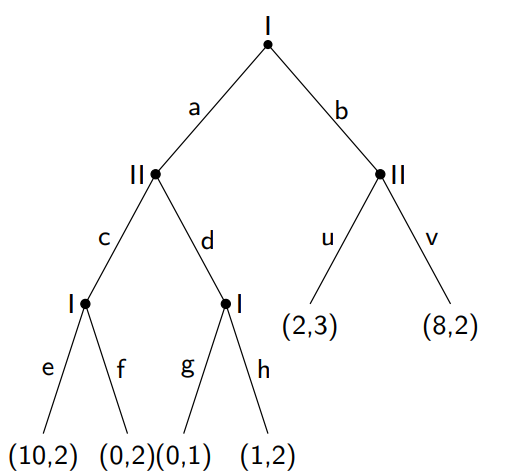
\includegraphics[width=0.75\linewidth]{images/tree2.png}
    \end{figure}
    The strategies in the tree are: 
    \begin{figure}[H]
        \centering
        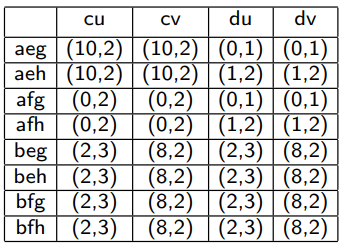
\includegraphics[width=0.75\linewidth]{images/strategies.png}
    \end{figure}
    Remember that the first player is in the rows, while the second is in the columns. 
    All combinations are listed even if equivalent (e.g. strategies b.. for Player II)
    The table has repeated pairs: different strategies can lead to the same outcomes
    \begin{itemize}
        \item Extensive form: the different moves of the players are presented in sequence
        \item Strategic form: all strategies of the players are presented at the same time
    \end{itemize}
\end{example}

\begin{theorem}[Von Neumann for strategies]
    In the chess game one of the following alternatives holds:
    \begin{enumerate}
        \item the white has a winning strategy.
        \item the black has a winning strategy.
        \item both players have a strategy leading them at least to a tie.
    \end{enumerate}
\end{theorem}
We have the first outcome if there is a raw with all winning elements. 
We have the second outcome if there is a column with all winning elements. 
The third outcome has a mixed outcomes, comprising also ties (but not all three outcomes in the same row or column). 

If $P_i = \{v_1, \dots, v_k \}$ and $v_j$ has $n_j$ children, then the number of strategies of Player $i$ is $n_1 \cdot n_2 \cdot \dots \cdot n_k$. 
This shows that the number of strategies even in short games is usually very high.
\begin{example}
    If Tic-Tac-Toe is stopped after three moves, the first player has (without exploiting symmetries) $9 \cdot 7 ^{(8\times9)}$ strategies
\end{example}

